% -*- TeX -*-
%
% ----------------------------------------------------------------------
%
%                           Brad T. Aagaard
%                        U.S. Geological Survey
%
% {LicenseText}
%
% ----------------------------------------------------------------------
%

\documentclass{beamer}
\usepackage{amsmath}

\title{PyLith Modeling Tutorial}
\subtitle{2-D Subduction Zone with \\
  Coseismic and Interseismic Deformation}
\author{Brad Aagaard \\
  Charles Williams \\
  Matthew Knepley}
\institute{
\includegraphics[scale=0.4]{../../logos/cig_blackfg}}
\date{June 17, 2016}


% ---------------------------------------------------- CUSTOMIZATION
\newcommand{\thispdfpagelabel}[1]{}
\newcommand{\important}[1]{{\bf\color{red}#1}}
\usetheme{CIG}

% ========================================================= DOCUMENT
\begin{document}

% ------------------------------------------------------------ SLIDE
\maketitle

% ------------------------------------------------------------ SLIDE
\logo{
\includegraphics[height=4.5ex]{../../logos/cig_blackfg}}

% ========================================================== SECTION
\section{Subduction Example}
\subsection{Overview}

% ------------------------------------------------------------ SLIDE
\begin{frame}
  \frametitle{2-D Subduction Zone Example}
  \summary{Features illustrated in this example}

  \begin{itemize}
  \item Generating a finite-element mesh using CUBIT
    \begin{itemize}
    \item Nonplanar geometry
    \item Variable mesh resolution
    \item Marking buried edges of faults
    \end{itemize}
  \item Spatially variable coseismic slip
  \item Maxwell viscoelastic relaxation
  \item Files are located in {\tt \color{red}
      src/pylith-2.1.2/examples/2d/subduction}
  \item {\tt Steps 1-2}: This tutorial
  \item {\tt Step 3-4}: Tinker time
  \end{itemize}
  
\end{frame}

% ------------------------------------------------------------ SLIDE
\begin{frame}
  \frametitle{2-D Subduction Zone Example}
  \summary{Based on 2011 M9.0 Tohoku, Japan, earthquake}

  \begin{center}
    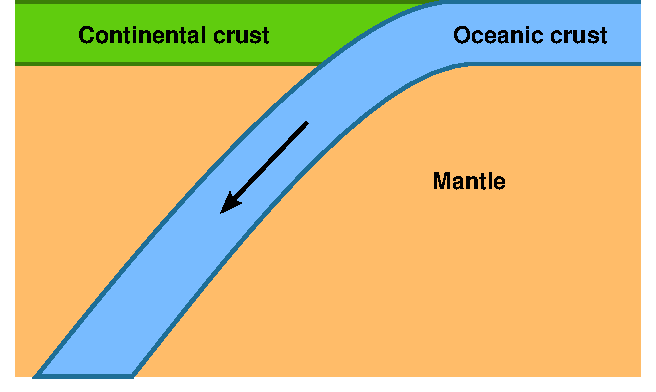
\includegraphics[scale=1.0]{figs/cartoon_general}
  \end{center}
  
\end{frame}

% ------------------------------------------------------------ SLIDE
\begin{frame}
  \frametitle{Steps in Subduction Zone Example}
  \summary{}

  \begin{center}
    \begin{tabular}{lc}
      \raisebox{0.48in}{Step01: Coseismic slip} & 
      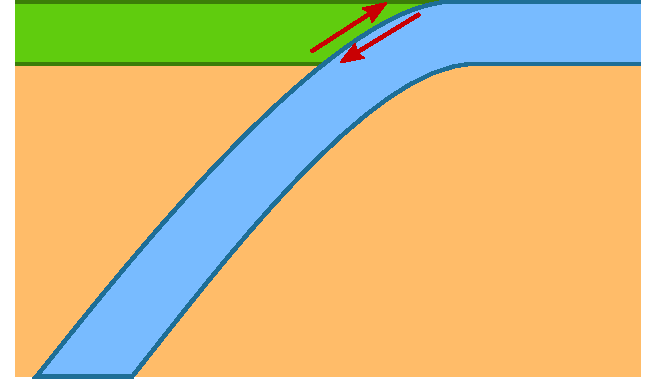
\includegraphics[height=0.95in]{figs/cartoon_step01} \\
      \raisebox{0.48in}{Step02: Interseismic deformation} &
      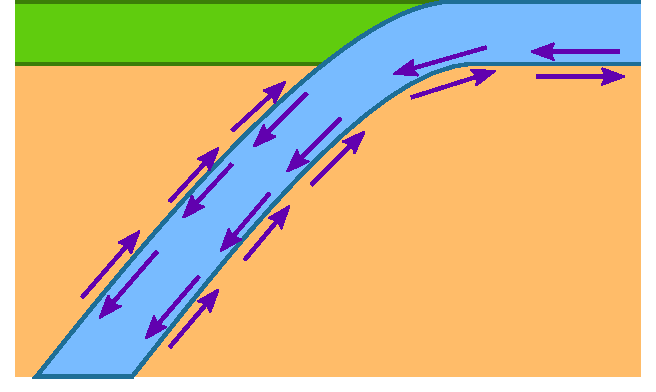
\includegraphics[height=0.95in]{figs/cartoon_step02} \\
      \raisebox{0.48in}{Step03: Seismic cycle} &
      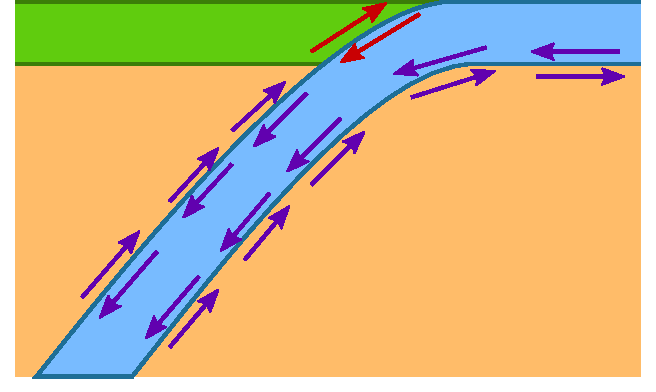
\includegraphics[height=0.95in]{figs/cartoon_step03}
    \end{tabular}
  \end{center}
  
\end{frame}


% ========================================================== SECTION
\subsection{General Parameters}

% ------------------------------------------------------------ SLIDE
\begin{frame}
  \frametitle{Parameters Common to All Steps}
  \summary{}
 
  \begin{itemize}
  \item Bulk constitutive models
    \begin{description}
    \item[Crust] Linear elastic w/plane strain (ElasticPlaneStrain)
    \item[Mantle] Linear Maxwell viscoelastic w/plane strain
      (MaxwellPlaneStrain)
    \end{description}
  \item Faults w/prescribed slip
  \item Fixed boundaries (except subducting slab)
  \end{itemize}

\end{frame}


% ========================================================== SECTION
\subsection{Mesh}

% ------------------------------------------------------------ SLIDE
\begin{frame}
  \frametitle{Mesh Generation via CUBIT}
  \summary{Include topography/bathymetry and slab geometry}
 
  \begin{enumerate}
  \item Create geometry
    \begin{enumerate}
    \item Create points
    \item Connect points into spline curves
    \item Split curves to form bounding curves
    \item Connect curves into surfaces
    \item Stitch surfaces together
    \end{enumerate}
  \item Define meshing scheme and cell size variation
    \begin{enumerate}
    \item Define cell size along curves near fault
    \item Increase cell size away from fault at geometric rate (bias)
    \end{enumerate}
  \item Generate mesh
  \item Create boundary conditions
  \item Export mesh
  \end{enumerate}
  
\end{frame}


% ========================================================== SECTION
\subsection{Step01}

% ------------------------------------------------------------ SLIDE
\begin{frame}
  \frametitle{Step01: Coseismic Slip}
  \summary{Prescribed slip based on Gavin Hayes's rupture model}
 
  \begin{center}
    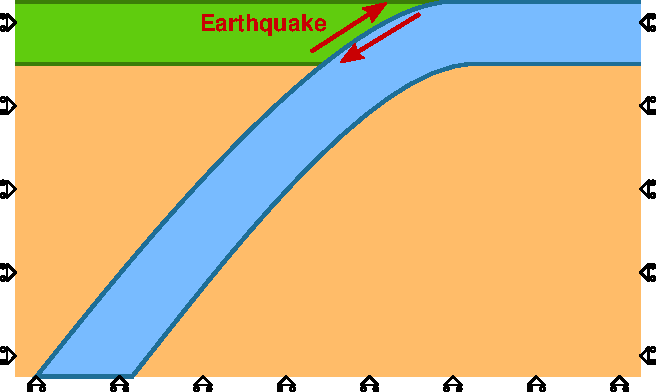
\includegraphics[scale=1.0]{figs/diagram_step01}
  \end{center}

\end{frame}


% ========================================================== SECTION
\subsection{Step02}

% ------------------------------------------------------------ SLIDE
\begin{frame}
  \frametitle{Step02: Interseismic Deformation}
  \summary{Aseismic creep along interface between slab and mantle}
 
  \begin{center}
    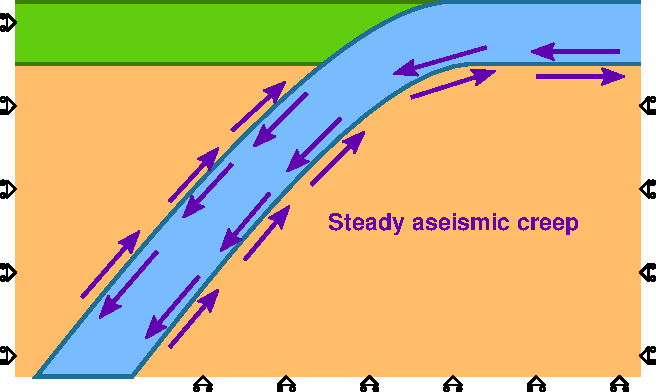
\includegraphics[scale=1.0]{figs/diagram_step02}
  \end{center}

\end{frame}


% ========================================================== SECTION
\subsection{Step03}

% ------------------------------------------------------------ SLIDE
\begin{frame}
  \frametitle{Step03: Seismic Cycle}
  \summary{Interseismic deformation with coseismic slip at 150 years}
 
  \begin{center}
    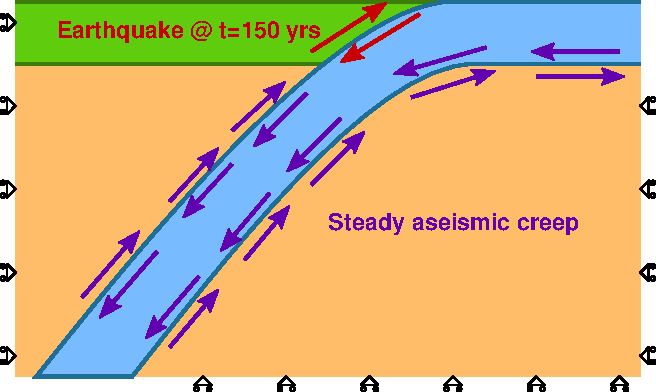
\includegraphics[scale=1.0]{figs/diagram_step03}
  \end{center}

\end{frame}


% ========================================================== SECTION
\subsection{Step05+}

% ------------------------------------------------------------ SLIDE
\begin{frame}
  \frametitle{Suggested Modifications}
  \summary{Examples of how to work towards real research problems}
 
  \begin{itemize}
  \item Add depth dependent viscosity to the mantle
  \item Add viscosity to the oceanic crust to permit relaxation at
    depths below 50 km
  \item Modify the spatial database files for the material properties
    to use depth-dependent elastic properties based on PREM
  \item Mesh the geometry using quad4 cells rather than tri3 cells
  \item Add multiple, repeated earthquake ruptures and examine spinup
    towards a steady-state solution
  \end{itemize}

\end{frame}


% ======================================================================
\end{document}


% End of file
